% Document configuration 

\documentclass{beamer}

\usepackage[utf8]{inputenc}
\usepackage{listings}
\usepackage{xcolor}
\usepackage{amsfonts}
\usepackage{graphicx}
\usepackage{wrapfig}

% Color definitions
\definecolor{codegreen}{rgb}{0,0.6,0}
\definecolor{codegray}{rgb}{0.5,0.5,0.5}
\definecolor{codepurple}{rgb}{0.58,0,0.82}
\definecolor{backcolour}{RGB}{240,240,240}

% Define a listing style
\lstdefinestyle{mystyle}{
  backgroundcolor=\color{backcolour}, commentstyle=\color{codegreen},
  keywordstyle=\color{magenta},
  numberstyle=\tiny\color{codegray},
  stringstyle=\color{codepurple},
  basicstyle=\ttfamily\footnotesize,
  breakatwhitespace=false,         
  breaklines=true,                 
  captionpos=b,                    
  keepspaces=true,                 
  numbers=left,                    
  numbersep=5pt,                  
  showspaces=false,                
  showstringspaces=false,
  showtabs=false,                  
  tabsize=2
}

% Set the listing style
\lstset{style=mystyle}

\usetheme{Madrid}

%--------------------------

% Title page setup

\title[Plataforma Digital]
{Logística Urbana para Entrega de Mercadorias}

\subtitle{Plataforma Digital}

\author[Grupo 30, 2LEIC03]
{Guilherme Sequeira, Pedro Ramalho, Tomás Pacheco}

\institute[FEUP]
{
  Faculdade de Engenheria\\
  Universidade do Porto
}

\date[2021/2022 2S]
{Desenho de Algoritmos, 2021/2022, 2º semestre}

%--------------------------

% Display the table of contents at the beginning of each section

\AtBeginSection[]
{
  \begin{frame}
    \frametitle{Conteúdos}
    \tableofcontents[currentsection]
  \end{frame}
}

%--------------------------

%----------------------------------------------

% START DOCUMENT

\begin{document}


% Initialize title page

\frame{\titlepage}


% Initialize table of contents

\begin{frame}
  \frametitle{Conteúdos}
  \tableofcontents
\end{frame}




%-------------------------------------------------------

% Begin section : Descrição do problema

\section{Descrição do problema}

%-------------------------------------------------------

% frame 1
\begin{frame}[fragile]
\frametitle{Descrição do problema}
O objetivo do projeto consiste em implementar a plataforma de uma empresa
de logística urbana, de modo a tornar a sua operação o mais eficiente possível.
Considera-se então a implementação de 3 cenários diferentes, cada um com o seu propósito.\\

A seguir apresenta-se uma explicação formal e detalhada sobre cada um destes cenários, bem como
as análises temporais da sua implementação.
\end{frame}

% End section : Descrição do problema

%-------------------------------------------------------




%-------------------------------------------------------

% Begin section : Cenário 1 - Minimização de Estafetas

\section{Cenário 1 - minimização de estafetas}

% frame 1
\begin{frame}
\frametitle{Formalização do problema}
\begin{block}{Descrição}
Dado um conjunto de estafetas $E$, de tamanho $m$, cada um com volume máximo $V_{e}$ e peso máximo $W_{e}$,
e um conjunto de pedidos $P$, de tamanho $n$, cada um com volume $v_{p}$ e peso $w_{p}$, pretende-se
maximizar o número de pedidos entregues, minimizando o número de estafetas contratados.  
\end{block}

Seja $I_{p}$ a variável que representa a inclusão da entrega $p \in P$, $C_{e}$ a variável que representa
a contratação do estafeta $e \in E$, e $x_{ep}$ a variável que determina se o pedido $p$ é entregue pelo estafeta $e$.\\

\begin{enumerate}
\setlength\itemsep{1em}
\item{Objetivo}

\textbf{maximizar} $ \sum_{p = 1}^{n} I_{p} $ 
\hspace{3cm} \textbf{minimizar} $ \sum_{e = 1}^{m} C_{e} $

\item{Restrições}
\begin{itemize}
  \item $ w_{p}, W_{e}, v_{p}, V_{e} \in \mathbb{Z}^{+}$  
  \item $ C, I, x \in \{ 0, 1 \} $
  \item $ W_{e} \geq \sum_{p = 1}^{n} w_{p}x_{ep}, $ $ V_{e} \geq \sum_{p = 1}^{n} v_{p}x_{ep} $
\end{itemize}

\end{enumerate}

\end{frame}

% frame 2
\begin{frame}[fragile]
\frametitle{Descrição do algoritmo}
Em baixo encontra-se pseudocódigo para o algoritmo usado no cenário 1:\\
\begin{lstlisting}[language=python]
sort(estafetas, ordem decrescente, por valor)
sort(pedidos, ordem decrescente, por valor)

for pedido in pedidos:
  for estafeta in estafetas:
    if pedido fits in estafeta:
      estafeta.add_pedido(pedido)
      break
\end{lstlisting}
\end{frame}

% frame 3
\begin{frame}
\frametitle{Análise da complexidade}
Relembrando que $m$ indica o número de estafetas e $n$ indica o número de pedidos, o algoritmo anterior
possui complexidade:\\ 
\centerline{$\mathcal{O}(nlog(n) + mlog(m) + mn)$}

\begin{figure}
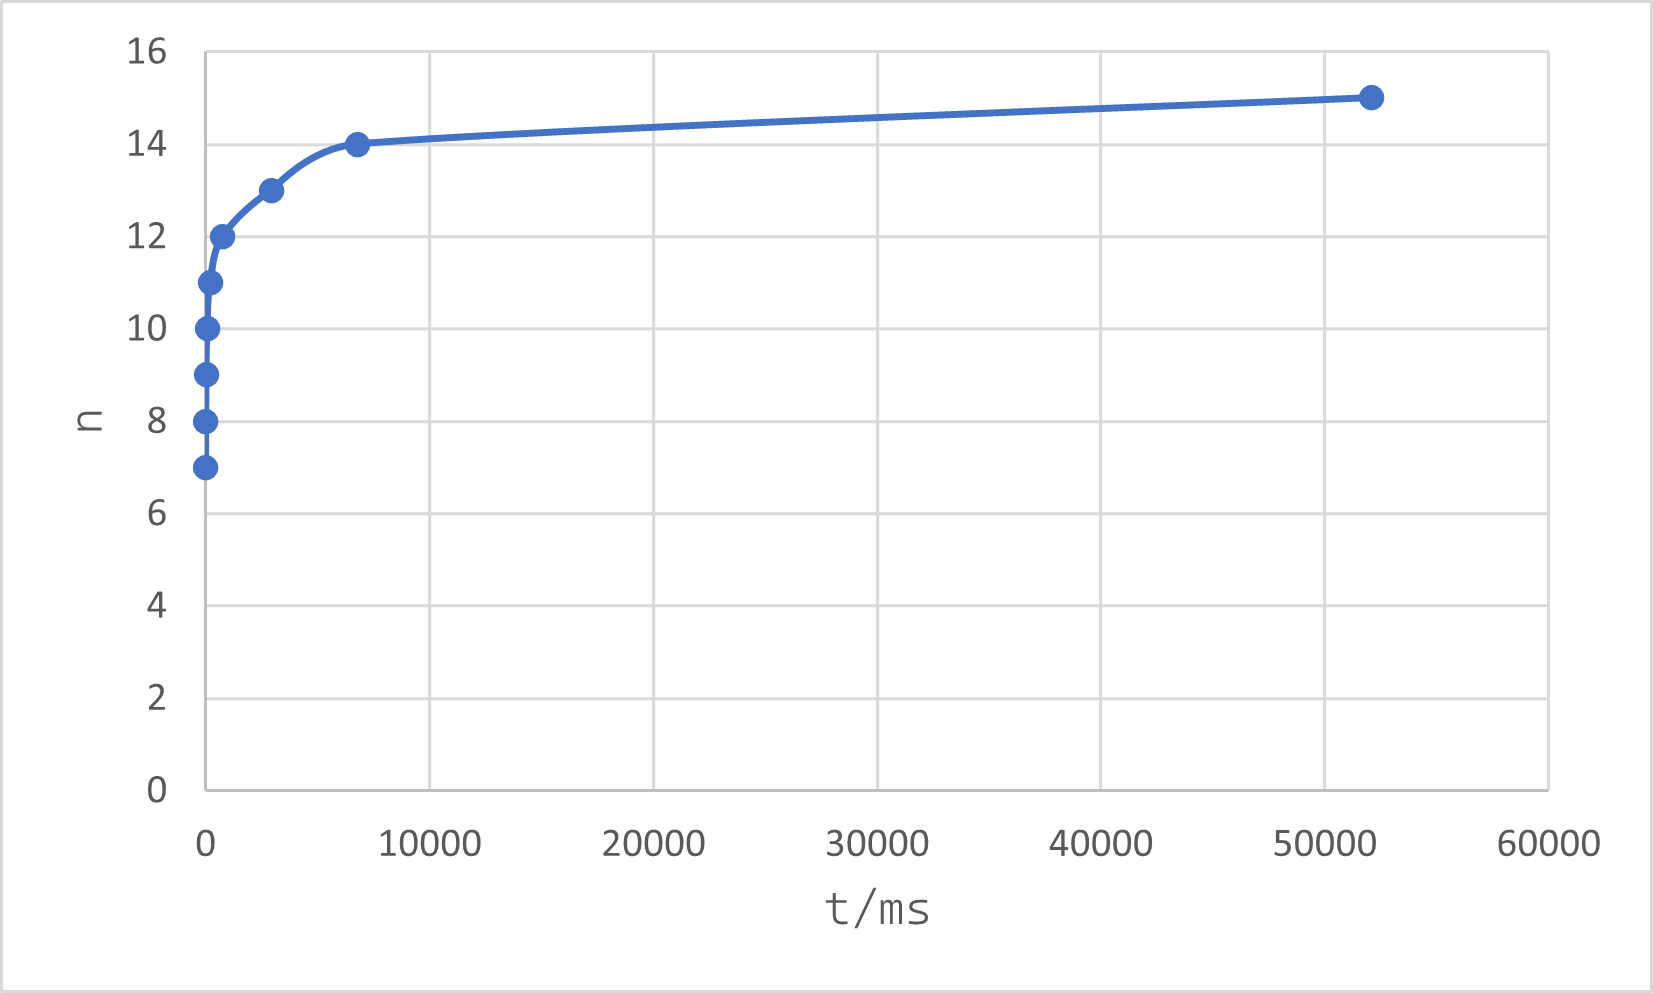
\includegraphics[width=0.5\linewidth]{assets/scenario1.png}
\end{figure}
{\scriptsize (n = 7, t = 4, e = 54) \hspace{0.1cm} (n = 8, t = 8, e = 107) \hspace{0.1cm} (n = 9, t = 21, e = 215)}\\
{\scriptsize (n = 10, t = 62, e = 422) \hspace{0.1cm} (n = 11, t = 198, e = 853) \hspace{0.1cm} (n = 12, t = 766, e = 1703)}\\
{\scriptsize (n = 13, t = 2927, e = 3402) \hspace{0.1cm} (n = 14, t = 6795, e = 6795) \hspace{0.1cm} (n = 15, t = 52077, e = 13576)}\\

{\footnotesize \textit{Observação: para um valor $n = k$ haverá $2^{k}$ estafetas e $ 9 \times 2^{k}$ pedidos.}}

\end{frame}

% frame 4
\begin{frame}
\frametitle{Resultados da avaliação empírica}
\begin{alertblock}{Problema}
É necessário atribuir um critério de prioridade aos estafetas e aos pedidos. Como obter tal critério?
\end{alertblock}

Inicialmente, começou-se por chamar a este critério de "valor". Assim, cada estafeta e pedido 
possui um valor associado.
A primeira iteração do algoritmo definia o valor de um estafeta e pedido da seguinte forma:\\
\centerline{$val_{e} = min(w_{e}/w_{t}, v_{e}/v_{t})$   \hspace{2cm}   $val_{p} = min(w_{p}/w_{t}, v_{p}/v_{t})$,}

onde $w_{t}$ e $v_{t}$ representam o peso e volume ocupado por todos os pedidos, respetivamente.

Desta forma, o algoritmo seria capaz de ajustar a prioridade dada aos estafetas selecionados de acordo com a necessidade de peso ou volume mais predominante nos pedidos.
Após várias iterações observou-se que $val_{e} = w_{e} + v_{e}$ e $val_{p} = w_{p} + v_{p}$ obteve os melhores resultados.
\end{frame}

% End section : Cenário 1 - Minimização de Estafetas

%-------------------------------------------------------




%-------------------------------------------------------

% Begin section : Cenário 2 - Maximização dos Lucros

\section{Cenário 2 - maximização dos lucros}

% frame 1
\begin{frame}
\frametitle{Formalização do problema}
\begin{block}{Descrição}
Dado um conjunto de estafetas $E$, de tamanho $m$, cada um com volume máximo $V_{e}$, peso máximo $W_{e}$ e custo $C_{e}$,
e um conjunto de pedidos $P$, de tamanho $n$, cada um com volume $v_{p}$, peso $w_{p}$ e recompensa $c_{p}$, pretende-se
maximizar o número de pedidos entregues de forma a maximizar os lucros da empresa.  
\end{block}

Seja $I_{p}$ a variável que representa a inclusão da entrega $p \in P$, $H_{e}$ a variável que representa
a contratação do estafeta $e \in E$, e $x_{ep}$ a variável que determina se o pedido $p$ é entregue pelo estafeta $e$.

\begin{enumerate}
\setlength\itemsep{1em}
\item{Objetivo}

\textbf{maximizar} $ \sum_{p = 1}^{n} I_{p} $ 
\hspace{1cm} \textbf{maximizar} $ \sum_{p = 1}^{n} c_{p}I_{p} - \sum_{e = 1}^{m} C_{e}H_{e} $

\item{Restrições}
\begin{itemize}
  \item $ w_{p}, W_{e}, v_{p}, V_{e}, c_{p}, C_{e} \in \mathbb{Z}^{+} $  
  \item $ I, H, x \in \{ 0, 1 \} $
  \item $ W_{e} \geq \sum_{p = 1}^{n} w_{p}x_{ep} $, $ V_{e} \geq \sum_{p = 1}^{n} v_{p}x_{ep} $
\end{itemize}

\end{enumerate}

\end{frame}

% frame 2
\begin{frame}[fragile]
\frametitle{Descrição dos algoritmos}
Em baixo encontra-se pseudocódigo para o algoritmo usado no cenário 2:\\
\begin{lstlisting}[language=python]
sort(estafetas, ordem decrescente, por custo)
sort(pedidos, ordem decrescente, por custo)

for pedido in pedidos:
  for estafeta in estafetas:
    if pedido fits in estafeta:
      estafeta.add_pedido(pedido)
      break
\end{lstlisting}
\end{frame}

% frame 3
\begin{frame}
\frametitle{Análise da complexidade}
Relembrando que $m$ indica o número de estafetas e $n$ indica o número de pedidos, o algoritmo anterior
possui complexidade:\\ 
\centerline{$\mathcal{O}(nlog(n) + mlog(m) + mn)$}

\begin{figure}
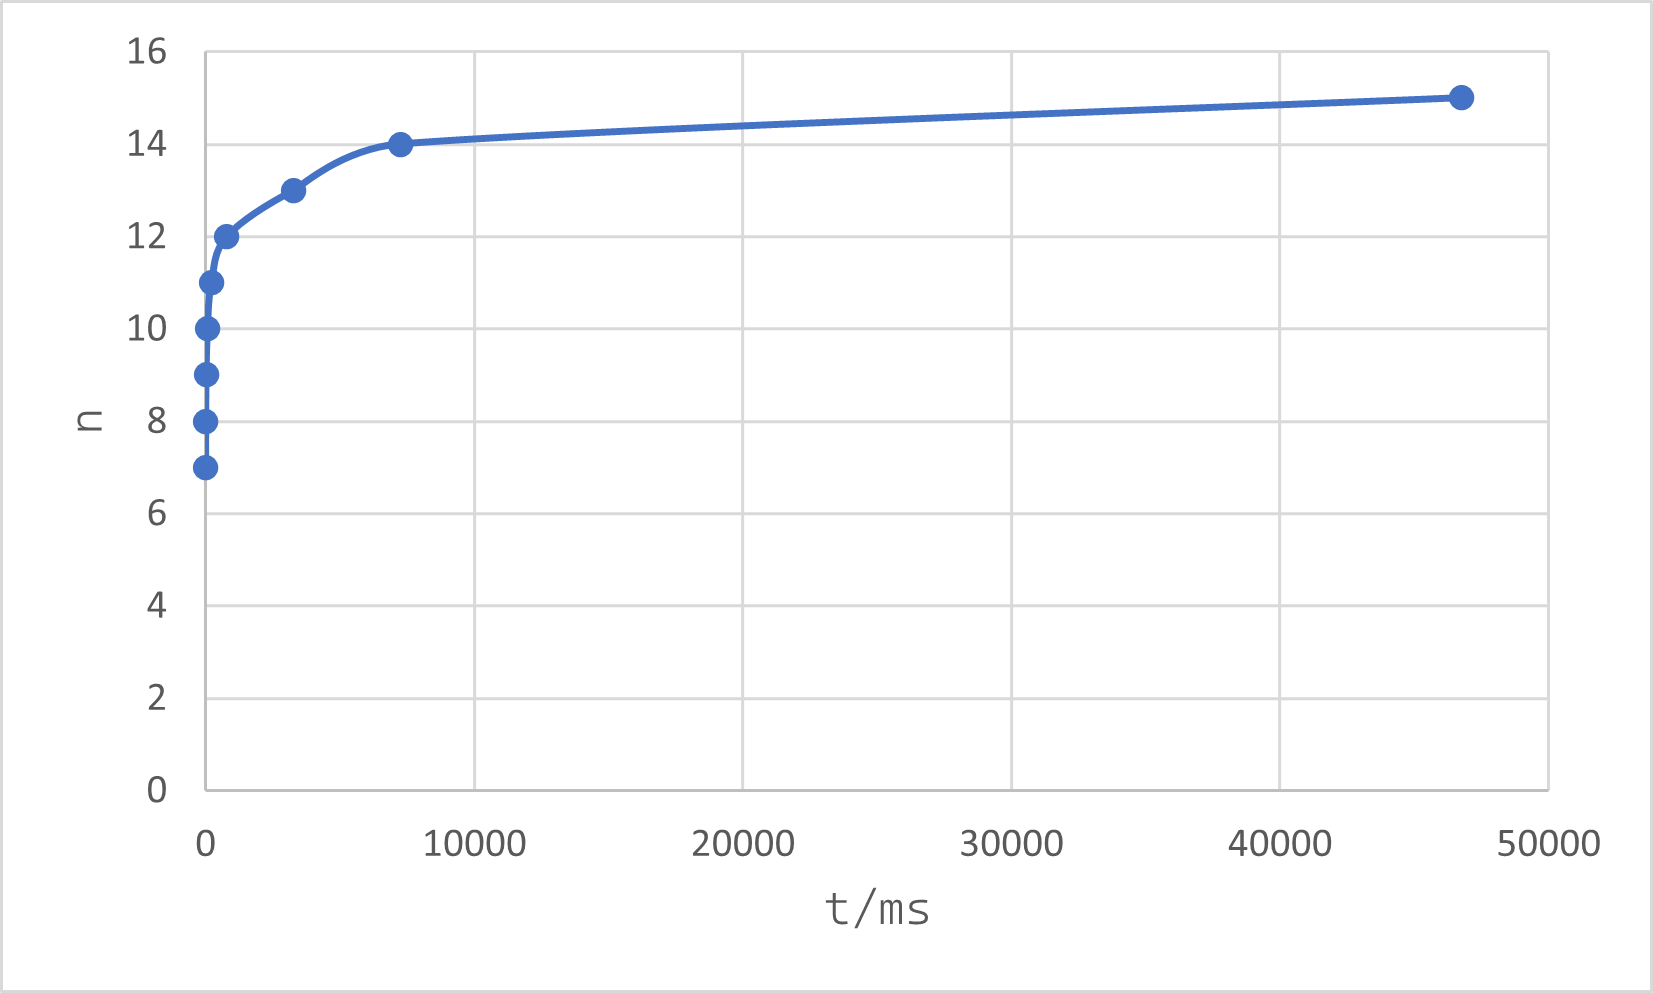
\includegraphics[width=0.5\linewidth]{assets/scenario2.png}
\end{figure}
{\tiny (n = 7, t = 3, L = 378472) \hspace{0.1cm} (n = 8, t = 8, L = 766746) \hspace{0.1cm} (n = 9, t = 19, L = 1415487)}\\
{\tiny (n = 10, t = 70, L = 2951155) \hspace{0.1cm} (n = 11, t = 217, L = 5963478) \hspace{0.1cm} (n = 12, t = 795, L = 12009077)}\\
{\tiny (n = 13, t = 3285, L = 23843787) \hspace{0.1cm} (n = 14, t = 7240, L = 48277534) \hspace{0.1cm} (n = 15, t = 46744, L = 96521460)}\\

{\footnotesize \textit{Observação: para um valor $n = k$ haverá $2^{k}$ estafetas e $ 9 \times 2^{k}$ pedidos.}}
\end{frame}

% frame 4
\begin{frame}
\frametitle{Resultados da avaliação empírica}
\begin{alertblock}{Problema}
É necessário atribuir um critério de prioridade aos estafetas e aos pedidos. Como obter tal critério?
\end{alertblock}

Inicialmente, começou-se por chamar a este critério de "custo". Assim, cada estafeta e pedido 
possui um custo associado.
A primeira iteração do algoritmo definia o custo de um estafeta e pedido da seguinte forma:\\
\centerline{$C_{e} = (W_{e} + V_{e})/R_{e}$   \hspace{1cm}   $c_{p} = r_{p}/(w_{p} + v_{p})$,}

onde $R_{e}$ e $r_{p}$ representam o custo de um estafeta e a recompensa de um pedido, respetivamente.

Desta forma, o algoritmo daria prioridade aos estafetas que possuissem uma capacidade de armazenamento maior, com um custo menor, e aos pedidos com uma recompensa maior, que ocupassem menos espaço.
Após várias iterações observou-se que $c_{p} = w_{p} + v_{p}$ obteve os melhores resultados.
\end{frame}

% End section : Cenário 2 - Maximização dos Lucros

%-------------------------------------------------------




%-------------------------------------------------------

% Begin section : Cenário 3 - Minimização do Tempo de Entrega

\section{Cenário 3 - minimização do tempo de entrega}

% frame 1
\begin{frame}
\frametitle{Formalização do problema}
\begin{block}{Descrição}
Dado um conjunto de pedidos \textit{expresso} $P$, de tamanho n, cada um com tempo de entrega $t_{p}$, pretende-se 
maximizar o número de pedidos entregues num só dia, sabendo que a entrega dos pedidos só pode ocorrer entre as 09:00h e 17:00 e só pode ser entregue um único pedido de cada vez.
\end{block}

Seja $I_{p}$ a variável que representa a inclusão da entrega $p \in P$.

\begin{enumerate}
\setlength\itemsep{1em}
\item{Objetivo}

\textbf{maximizar} $ \sum_{p = 1}^{n} I_{p} $ 

\item{Restrições}
\begin{itemize}
  \item $ I \in \{ 0, 1 \} $
  \item $ \sum_{p = 1}^{n} I_{p}t_{p} \leq 8 \times 60 \times 60 $
\end{itemize}

\end{enumerate}

\end{frame}

% frame 2
\begin{frame}[fragile]
\frametitle{Descrição dos algoritmos}
Em baixo encontra-se pseudocódigo para o algoritmo do cenário 3:
\begin{lstlisting}[language=Python]
TEMPO_LIMITE = 8 * 60 * 60
tempo_total = 0
i = 0

sort(pedidos, ordem crescente, por tempo de entrega)

while true:
  entregar(pedido[i])
  tempo_total += pedido[i].tempo

  if tempo_total > TEMPO_LIMITE:
    tempo_total -= pedido[i].tempo
    retirar(pedido[i])
    break

  i++
\end{lstlisting}
\end{frame}

% frame 3
\begin{frame}
\frametitle{Análise da complexidade}
Relembrando que $n$ indica o número de pedidos, o algoritmo anterior
possui complexidade: \\
\centerline{$\mathcal{O}(nlog(n))$, no pior dos casos}

\begin{figure}
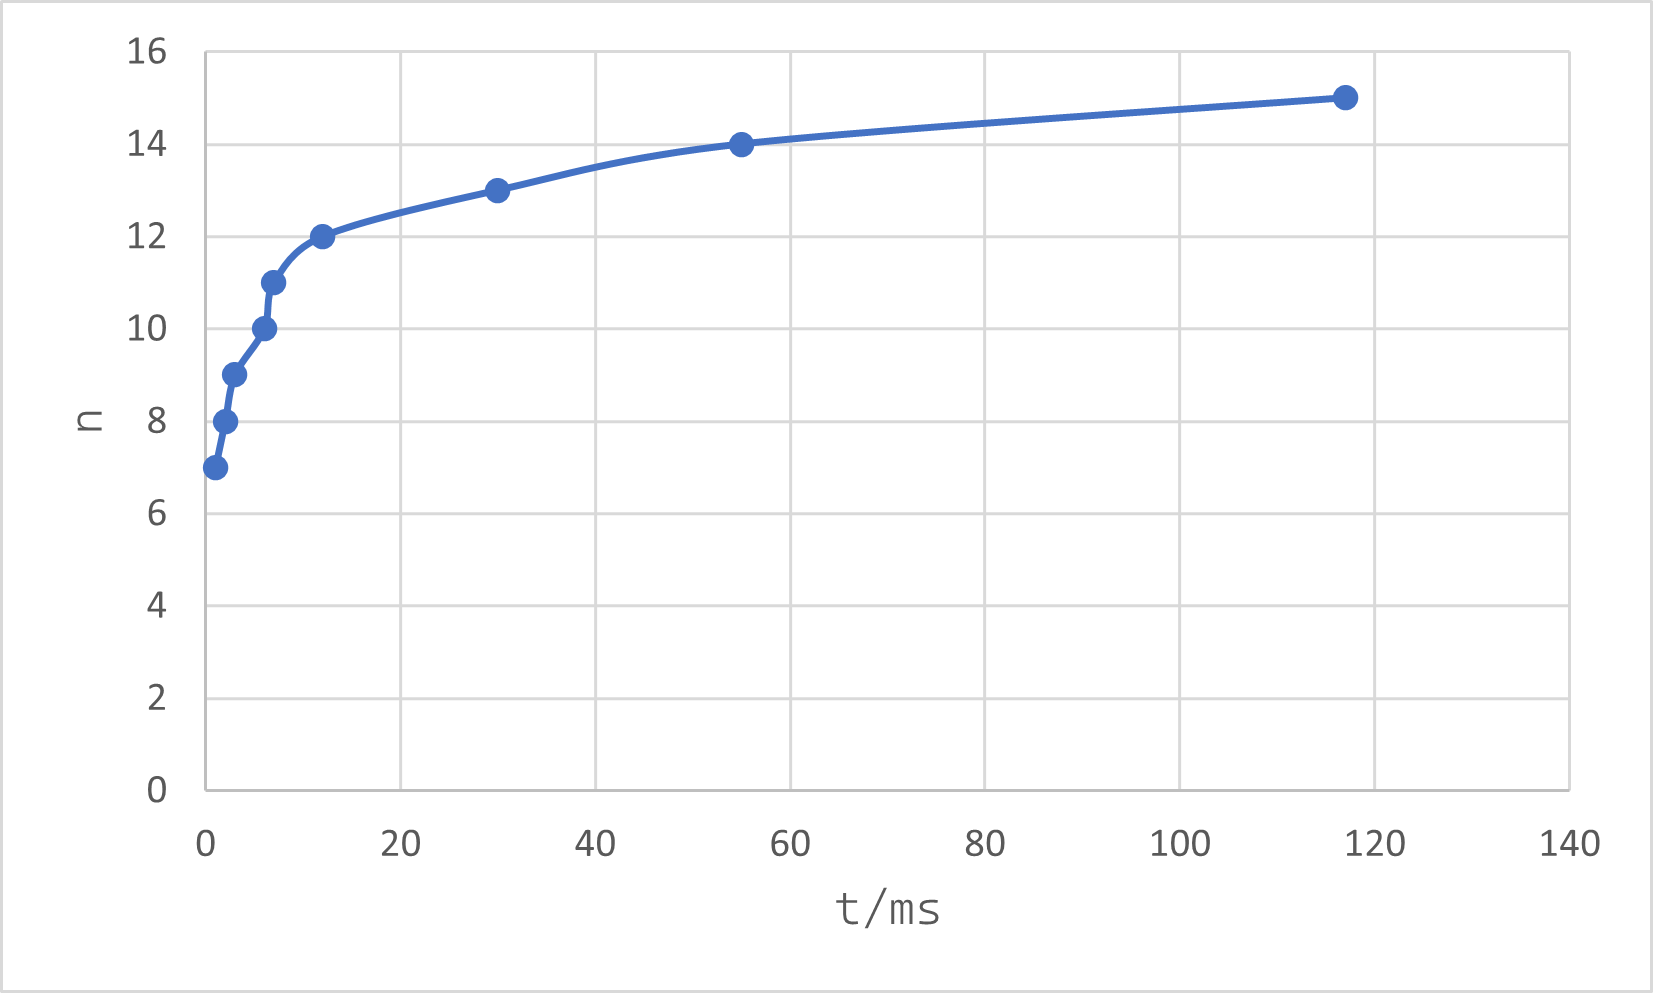
\includegraphics[width=0.5\linewidth]{assets/scenario3.png}
\end{figure}
{\scriptsize (n = 7, t = 1, p = 172) \hspace{0.1cm} (n = 8, t = 2, p = 202) \hspace{0.1cm} (n = 9, t = 3, p = 229)}\\
{\scriptsize (n = 10, t = 6, p = 254) \hspace{0.1cm} (n = 11, t = 7, p = 269) \hspace{0.1cm} (n = 12, t = 12, p = 278)}\\
{\scriptsize (n = 13, t = 30, p = 284) \hspace{0.1cm} (n = 14, t = 55, p = 286) \hspace{0.1cm} (n = 15, t = 117, p = 288)}\\

{\footnotesize \textit{Observação: para um valor $n = k$ haverá $2^{k}$ estafetas e $ 9 \times 2^{k}$ pedidos.}}
\end{frame}

% frame 4
\begin{frame}
\frametitle{Resultados da avaliação empírica}
A estratégia usada consiste em ordernar os pedidos por ordem crescente de duração, o que garante a solução ótima.
É uma abordagem \textit{greedy} ao problema que atinge os resultados esperados.
\end{frame}

% End section : Cenário 3 - Minimização do Tempo de Entrega

%-------------------------------------------------------




%-------------------------------------------------------

% Begin section : Destaque de Algoritmo

\section{Destaque de algoritmo}

% frame 1
\begin{frame}[fragile]
\frametitle{Destaque de algoritmo}
Os cenários 1 e 2 possuem soluções semelhantes - implementam um algoritmo de \textit{first-fit} em que os estafetas e pedidos foram sujeitos a uma heurística de ordenação de modo a maximizar a eficiência do mesmo.
O critério de prioridade, em cada cenário, provém de uma avaliação empírica resultante de diversas iterações de cada um dos algoritmos, pelo 
que sofreu várias alterações ao longo da realização do projeto.

Realça-se deste modo a obtenção de uma solução, para os primeiros cenários, que tenta emular o comportamento de um algoritmo \textit{first-fit decreasing} num contexto multi-dimensional.
\end{frame}

% End section : Destaque de Algoritmo

%-------------------------------------------------------



%-------------------------------------------------------

% Begin section : Principais dificuldades

\section{Principais dificuldades, esforço do grupo}

% frame 1
\begin{frame}
\frametitle{Principais dificuldades}
Durante a realização do projeto surgiram diversas dificuldades, pelo que se salientam as seguintes:
\begin{itemize}
  \item encontrar um critério de prioridade para os estafetas e pedidos, nos cenários 1 e 2
  \item o enquadramento de algoritmos conhecidos (\textit{bin-packing, 0-1 knapsack}) num contexto a 2 e 3 dimensões
  \item o estudo fidedígno e preciso da complexidade, quer temporal quer espacial, dos algoritmos implementados
\end{itemize}
Cada um dos elementos do grupo contribuiu equitativamente para a realização do projeto.
\end{frame}

% End section : Principais dificuldades

%-------------------------------------------------------




%-------------------------------------------------------

% Begin section : Outras observações

\section{Outras observações}

% frame 1
\begin{frame}
\frametitle{Como foi gerado o \textit{dataset}?}
Foram gerados um total de 9 ficheiros para estafetas e 9 ficheiros para entregas.
Estes dados foram obtidos da seguinte forma:

\begin{enumerate}
  \item definiu-se o número de estafetas numa potência de 2
  \item decidiu-se que o número de entregas seria 9 vezes o número de estafetas, de modo a ser fiel ao \textit{dataset} original
  \item geraram-se valores aleatórios para cada um dos atributos que compõe um estafeta e pedido (volume, peso, custo, recompensa, tempo...)
  \item escreveram-se os dados em ficheiros com a mesma formatação do \textit{dataset} original
\end{enumerate}

Caso o utilizador queira usar o seu próprio dataset deverá garantir que o ficheiro dos estafetas e pedidos
possuem exatamente os nomes \textit{assistants.txt} e \textit{deliveries.txt}, respetivamente.
Deverá ainda garantir que a primeira linha de cada ficheiro contém o número de linhas com informação a ser processada pela plataforma.

\end{frame}

%frame 2
\begin{frame}
\frametitle{Oportunidades de melhoria}
Os critérios de prioridade escolhidos para os cenários 1 e 2 derivam essencialmente de um processo de tentativa e erro.
No entanto, podem existir formas de melhorar os resultados obtidos para estes algoritmos, pelo que se salientam as seguintes:
\begin{enumerate}
  \item um critério de ordenação que melhor se adaptasse à natureza bi ou tridimensional do problema, ou seja, que desse igual importância às variáveis envolvidas sem as tratar de forma intercambiável, como é o caso do volume e do peso
  \item uma melhor atribuição de pedidos a um estafeta, que tenha em conta o contexto global do cenário, de modo a aprimorar os resultados obtidos
  \item experimentação com outras tácticas de inserção de pedidos em estafetas, como por exemplo \textit{knapsack} binário bidimensional
\end{enumerate}
\end{frame}

% End section : Outras observaçṍes

%-------------------------------------------------------

\section{Referências}

% frame 1
\begin{frame}
\frametitle{Referências}
Referências:\\
https://www.sciencedirect.com/science/article/abs/pii/S0167637703000579
https://www.sciencedirect.com/science/article/pii/S1877050913003980
\end{frame}

\end{document}
